\section{Go kalbos priklausomybių valdymo sistema}

Go programavimo kalboje (dar žinomoje kaip Golang), numatytasis priklausomybių valdymo įrankis yra „go get“
komanda. Naudodamasis šia komanda, vartotojas gali atsisiųsti vystomam projektui reikalingas priklausomybes.
Ateinančiuose skyriuose aptariami naujausi „go get“ pokyčiai ir šių pokyčių atnešami privalumai.

\subsection{Priklausomybių valdymo Go kalboje istorija}

Nuo pat Go kalbos išleidimo 2009 metais, jos naudotojų tarpe atsirado poreikis dalintis savo, bei naudoti kitų vartotojų sukurtus paketus.
Šiam tikslui Go inžinieriai sukūrė „GOINSTALL“ komandą, leidžiančią atsisiųsti norimus paketus iš tokių programinio kodo saugyklų kaip Github ar Bitbucket.
Neilgai trukus „GOINSTALL“ pakeitė “go get“ komanda, tačiau abi šios komandos turėjo didžiulį trūkumą - jose nebuvo
paketo versijos sąvokos. Tai reiškė, jog naudojant „go get“ vartotojas visada gaus naujausią šio paketo kopiją \cite{COX18a}.

Negalėjimas pasirinkti paketo versijos kelia dvi pagrindines problemas.
Pirmoji problema yra negalėjimas užtikrinti stabilaus programos surinkimo (ang. stable build),
antroji - nėra galimybių užtikrinti, kad pokyčiai naujoje paketo versijoje bus atgaliai suderinami (ang. backwards-compatible).

Go priklausomybių valdymo trūkumai bandyti spręsti kopijuojant atsiųstus paketus ir laikant juos lokaliai -
šį procesą automatizuoti sukurta daug įrankių, tokių kaip goven, godep, gb. Lokalus paketų laikymas
išsprendė tik stabilaus programos surinkimo (ang. stable build) problemą. Priklausomybių versijų
atgalinio suderinamumo problema vis dar nebuvo išspręsta \cite{COX18a}.

Go kalboje buvo poreikis įvesti tiesioginį paketų versijų valdymą pačioje „go get“ komandoje ir nebepasikliauti trečiųjų šalių
įrankiais. Taip Go inžinieriai pradėjo dirbti prie Vgo - pirmojo apie priklausomybių versijas žinančios (ang. version-aware) Go
komandos prototipo \cite{COX18b}. Go kalbos 1.11 versijoje pradėtas pirminis Vgo prototipe pristatytų idėjų palaikymas
\cite{GOLANG19}.


\subsection{Priklausomybių versijavimas Go sistemoje}

Go inžinierių pasiūlymas dėl version-aware Go komandos implementacijos apsprendžia, kaip naujoje
Go bus versijuojamos priklausomybės. Trečiasis šio pasiūlymo punktas nurodo, kad atnaujintoje Go bus
naudojamas semantinis importų versijavimas (ang. semantic import versioning) \textsuperscript{[COX18c]}.
Semantiniu importų versijavimu siekiama, jog su kiekvienam atgaliai nesuderinamui paketo pakeitimui bus priskiriamas
skirtingas importavimo kelias (ang. import path) su specifikuota pagrindine (ang. major) versija, pavyzdžiui, “github.com/greta/foo/v2".

\begin{figure}[H]
    \centering
    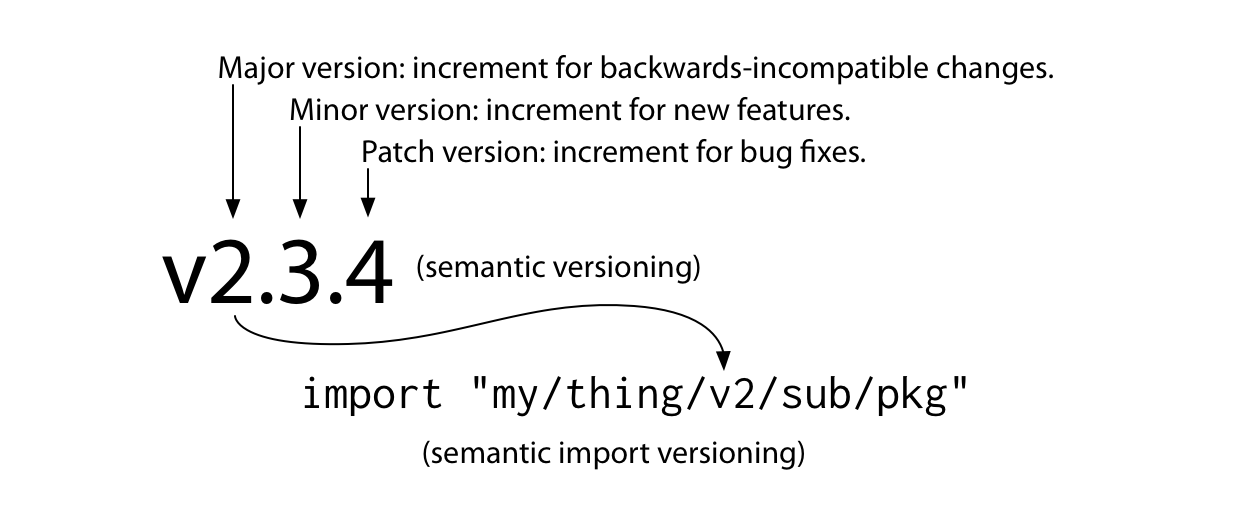
\includegraphics[width=\textwidth]{semantic_import_versioning}
    \caption{Semantinis importų versijavimas \textsuperscript{[COX18d]}}
\end{figure}

Ketvirtasis Go pasiūlymo punktas, importų suderinamumo taisyklė, papildo prieš
tai pasiūlyme pristatytą semantinio importų versijavimo idėją. Ši taisyklė teigia: jei
senas paketas ir naujas paketas turi tą patį importavimo kelią, tuomet naujas paketas privalo būti atgaliai
suderinamas su senuoju \textsuperscript{[COX18c]}.Importų suderinamumo taisyklė paketų autoriams nustato griežtas ribas, kokie pakeitimai leidžiami
nekeičiant paketo importavimo kelio ir kokius pakeitimus įvykdžius būtina kurti naują importavimo kelią.

Naudojant semantinį paketų versijavimą bei laikantis importų suderinamumo taisyklės tikimasi išspręsti prieš tai „go get“
komandoje buvusią nestabilaus API problemą - paketų naudotojams suteikiama garantija,
kad atnaujinant priklausomybes jų naudojamų paketų metodai nesikeis.


\subsection{Priklausomybių versijų pasirinkimas Go sistemoje}

Nuo pat „go get“ pristatymo, viena didžiausių šios komandos problemų buvo
nežinojimas apie valdomų paketų versijas.
Senoji „go get“ komanda turėjo du priklausomybių versijų pasirinkimo algoritmus.
Pirmasis, Go numatytasis algoritmas, „go get B“ metu atsiųsdavo naujausią paketo B versiją
bei naujausias B priklausomybes, kurių nebuvo turima lokaliai. Antrasis algoritmas įvykdžius „go get -u B“
atsiųsdavo naujausią B, bei visas naujausias jos tranzityvių priklausomybių versijas \cite{COX18d}.

Abu šie algoritmai netenkino vartotojų bei kėlė daug klaidų. Naudojant pirmąjį algoritmą,
kilo grėsmė, jog lokaliai turimos priklausomybės bus per senos ir neveiks su naujai atsiųstomis
priklausomybėmis. Antrasis algoritmas taip pat nebuvo visiškai saugus, nes buvo galimybė,
jog naujausios priklausomybių versijos nebus tarpusavyje sutapatinamos (ang. compatible) \cite{COX18e}.

%\begin{figure}[H]
%    \centering
%    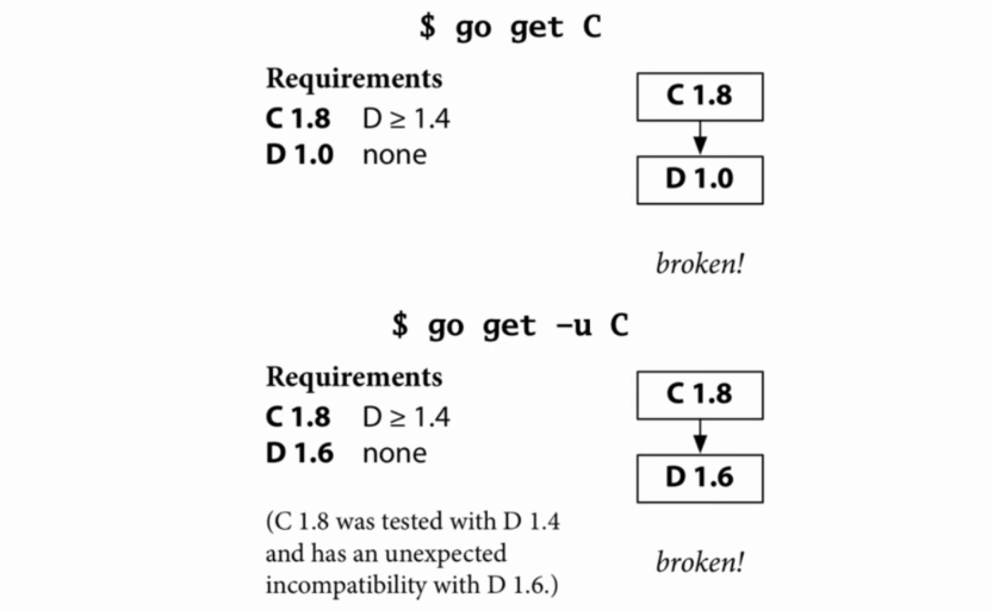
\includegraphics[width=\textwidth]{old_go_get}
%    \caption{Problemos „go get“ komandoje \textsuperscript{[COX18e]}}
%\end{figure}

Suprasdami „go get“ priklausomybių versijų pasirinkimo algoritmų keliamas problemas,
Go inžinieriai į pasiūlymą dėl version-aware Go komandos įtraukė ir naują algoritmą priklausomybių
versijų pasirinkimui. Šis algoritmas vadinasi „minimal version selection“ ir siūlo lyg šiol mažai naudotą
priklausomybių versijų pasirinkimo mechanizmą - pasirinkti seniausią leidžiamą paketo versiją.
Dauguma šiuolaikinių priklausomybių valdymo sistemų, tokių kaip dep ar cargo, naudoja priešingą algoritmą -
renkasi naujausią leidžiamą priklausomybės versiją \cite{COX18a} \cite{COX18f}.

Russ Cox, vienas pagrindinių Go kūrėjų, teigia, cargo bei dep naudojamas algoritmas yra klaidingas
dėl dviejų priežasčių. Pirmoji priežastis yra tai, jog naujausia leidžiama versija gali nuolat kisti
bei būti nestabili, antroji - klaidos atveju vartotojui reikia skirti papildomo
laiko uždrausti naudoti specifinių versijų priklausomybes \cite{COX18a}.

%\begin{figure}[H]
%    \centering
%    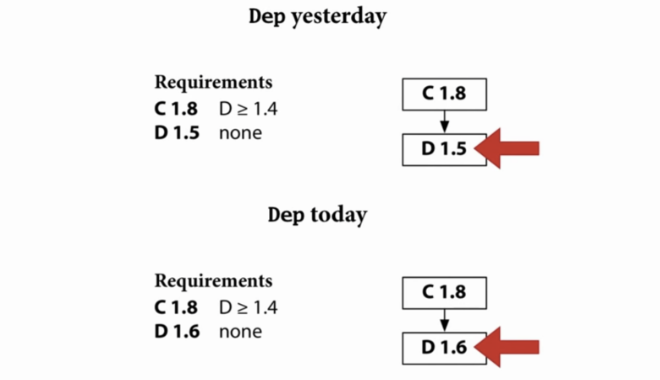
\includegraphics[width=\textwidth]{dep_working}
%    \caption{Naujausios leidžiamos versijos algoritmas dep sistemoje \textsuperscript{[COX18e]}}
%\end{figure}

Go inžinierių pasirinktas „minimal version selection“ algoritmas turi kelis pranašumus.
Šis algoritmas užtikrina, jog visada su ta pačia „go get“ komanda bus gaunamos tų pačių versijų priklausomybes.
Garantija, jog projekto priklausomybės nesikeis, leidžia užtikrinti, jog programos surinkimo rezultatas visada bus toks pats,
tiek programų sistemos kūrimo metu, tiek sistemos produkcinėje aplinkoje \cite{COX18a}. „Minimal version selection“ taip pat
leidžia apsisaugoti nuo naujausiose paketų versijose galinčių būti klaidų - jei paketo A naujausiose versijoje yra klaida,
tiek A paketo autorius, tiek kitų paketų, naudojančių A, autoriai turi laiko ištaisyti klaidą bei
uždrausti naudoti šią trikį turinčią versiją \cite{COX18e}.

%\begin{figure}[H]
%    \centering
%    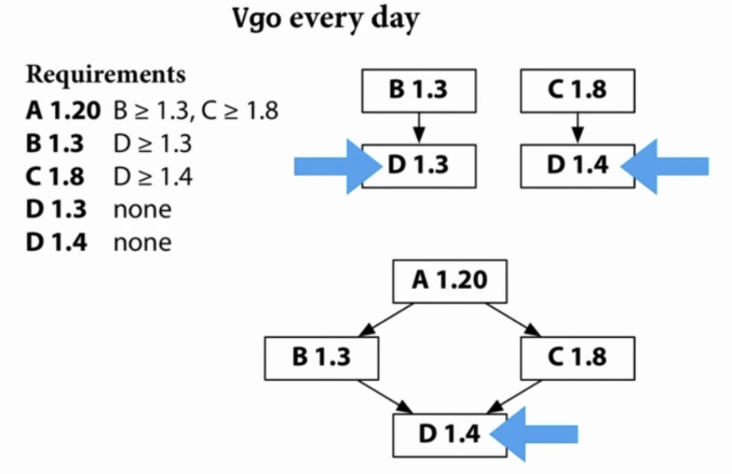
\includegraphics[width=\textwidth]{vgo_min_version}
%    \caption{„Minimal version selection“ \textsuperscript{[COX18e]}}
%\end{figure}


\section{NPM priklausomybių valdymo sistema}

NPM yra priklausomybių valdymo sistema, naudojama JavaScript aplikacijose.
Ši sistema turi didžiausią priklausomybių registrą pasaulyje, ja naudojantis galima atsisiųsti paketus arba Node modulius.

\subsection{Priklausomybių versijavimas NPM sistemoje}

NPM priklausomybėms versijuoti naudojama semantinio versijavimo sistema. Ši sistema versijuojamui vienetui
suteikia X.Y.Z formos versiją, kurioje X reiškia pagrindinę (ang. major) versiją, Y - antraeilę (ang. minor) versiją,
Z - pataisymų (ang. patch) versiją. Pataisymų (ang. patch) ir antraeilių (ang. minor) versijų pasikeitimai yra atgaliai suderinami
ir yra saugūs naudoti projektuose su ta pačia pagrindine (ang. major) versija \textsuperscript{[NPMb]}.
Tuo tarpu pagrindinės versijos pasikeitimas reiškia atgaliai nesuderinamus pokyčius.
Semantinis versijavimas leidžia vartotojui susidaryti lūkesčius naujoms priklausomybių versijoms bei
package.json faile apibrėžti kurios priklausomybių versijos ir kurie jų atnaujinimai yra leidžiami projekte.
Ši versijavimo sistema išsprendžia nestabilaus API problemą. %elaborate gurl


%\section{Priklausomybių valdymo sistemų analizė}
%
%\subsection{Vgo priklausybių valdymo sistema}
%
%Vgo yra Go programavimo kalbos (dar žinomos kaip Golang) priklausomybių valdymo sistema. Ši sistema Go inžinierių komandos pradėta kurti 201X, su tikslu pakeisti begalę prieš tai paplitusių trečiųjų šalių Go priklausomybių valdymo sistemų bei išspręsti šių sistemų keliamas problemas. Russ Cox, vienas iš pagrindinių Vgo kūrėjų, savo kalbose mini dar vieną Vgo siekiamybę - palengvinti programų sistemų kūrimo procesą.
%
%\bigbreak
%{\bf Istorija}
%\bigbreak
%
%Nuo pat Go kalbos išleidimo 2009 metais, jos naudotojų tarpe atsirado poreikis dalintis savo, bei naudoti kitų sukurtus paketus. Šiam tikslui Go inžinieriai sukūrė GOINSTALL komandą, leidžiančią atsisiųsti norimus paketus iš tokių programinio kodo saugyklų kaip Github ar Bitbucket. Neilgai trukus GOINSTALL pakeitė GO GET komanda, tačiau abi šios komandos turėjo didžiulį trūkumą - jose nebuvo paketo versijos sąvokos. Tai reiškė, jog naudojant GO GET vartotojas visada gaus naujausią šio paketo kopiją. Negalėjimas pasirinkti paketo versijos kelia dvi pagrindines problemas - nėra galimybės užtikrinti stable builds, taip pat nėra galimybės užtikrinti, kad pokyčiai naujojoje versijoje bus backwards-compatible. Šis Go priklausomybių valdymo trūkumas bandytas spręsti kopijuojant atsiųstus paketus ir laikant juos lokaliai - šį procesą automatizuoti sukurta daug įrankių, tokių kaip goven, godep, gb. Visgi lokalus paketų laikymas išsprendė tik stable builds problemą, priklausomybių versijų backwards-compatibility problema vis dar nebuvo išspręsta. Buvo aišku, jog būtina reikia įvesti tiesioginį paketų versijų pačioje Go komandoje ir nebepasikliauti trečiųjų šalių įrankiais. Taip Go inžinieriai 201X metais pradėjo dirbti prie Vgo - pirmojo bandymo sukurti version-aware Go komandą.
%
%\bigbreak
%{\bf Vgo principai}
%\bigbreak
%
%Go inžinierių pasiūlymą dėl version-aware GO komandos sudaro keturi žingsniai: importavimo suderinamumo taisyklė (ang. the import compatibility rule), minimalios versijos pasirinkimas (ang. minimal version selection), nauja Go module paketų rinkinio sąvoka bei  apsprendimas, kaip prieš tai minimus pakeitimus įdiegti į jau egzistuojančią Go komandą.
%
%\bigbreak
%{\bf Importavimo suderinamumo taisyklė}
%\bigbreak
%
%Importavimo suderinamumo taisyklė, pirmasis žingsnis į version-aware Go, teigia :
% jei senas paketas ir naujas paketas turi tą patį import path, tuomet naujas paketas privalo būti backwards-compatible su senuoju. Taip pat įvedamas semantinis import versioning - tikimasi, jog su kiekvienam backwards-incompatible paketo pakeitimui bus skirtingi import path su specifikuota major versija, pvz, import "github.com/greta/foo/v2". Šiais naujais reikalavimais tikimasi prieš tai GO GET komandoje buvusią unstable api problemą - paketų naudotojams suteikiama garantija, kad atsinaujinant priklausomybes jų naudojamų paketų metodai nesikeis.
%
%\bigbreak
%{\bf Minimalios versijos pasirinkimas}
%\bigbreak
%
%Daug priklausomybių valdymo sistemų, tokių taip dep ar npm,  siųsdamos priklausomybes pasirenka naujausią galimą paketo minimalią versiją. Senoji GO GET komanda taip pat automatiškai gaudavo tik naujausias priklausomybių versijas. Tokiose sistemose nėra garantijų, jog du kartus prasukus tą pačią paketų gavimo komandą bus gautas tos pačios versijos paketas. Tai reiškia, jog jei naujausioje A paketo versijoje 2.3.5 bus klaida, A paketą naudojantys paketai privalės greitai reaguoti ir uždrausti naudoti šią A paketo versiją. Taigi, toks naujausios minimalios versijos algoritmas buvo neprognozuojamas bei neapsaugojo paketo naudotojos nuo netikėtų klaidų. Go inžinieriai, norėdami išspręsti šių sistemų keliamas problemas nusprendė VGO naudoti kitą priklausomybių versijų pasirinkimo algoritmą - t.y. pasirinkti ne naujausią, o seniausią leidžiamą paketo minimalią versiją. Toks algoritmas užtikrina, kad visada su ta pačia komanda bus gaunamos tų pačių versijų priklausomybės. Taip pat jei paketo A naujausiose versijoje yra klaida, tiek paketo autorius, tiek kitų paketų, naudojančių A, autoriai turi laiko ištaisyti klaidą bei uždrausti naudoti šią versiją.
%
%\bigbreak
%{\bf Go Module}
%\bigbreak
%
%Vgo sistemoje įvedama Go modulio sąvoka - Go modulis apibūdinamas kaip paketų rinkinys, turintis bendrą import path prefiksą. Modulis taip pat yra versijavimo vienetas, tai reiškia, jog naudojantis vgo komanda galima gauti tik modulius, o ne atskirus paketus. Go moduliui galima taikyti minimalių versijų reikalavimus moduliams, nuo kurių jis priklauso - tai leidžia reaguoti į naujausiųjų modulių versijų klaidas bei neatitikimus ir kurti taisykles dėl leidžiamų modulių versijų.
%
%\bigbreak
%{\bf Apibendrinimas}
%\bigbreak
%
%Vgo priklausomybių valdymo sistema yra didelis patobulėjimas nuo prieš tai Go kalboje naudojamų įrankių, tokių kaip version-unaware go get, dep, goven. Netradicinis sprendimas sistemoje naudoti seniausios leidžiamos minimalios versijos pasirinkimo algoritmą leidžia išvengti netikėtų gedimų bei duoda laiko modulių kūrėjams išspręsti kilusias klaidas. Import compatibility taisyklė leidžia išspręsti ligi šiol buvusią skaudžią api instability problemą - tai pasiekta keliant griežtus reikalavimus Go modulių kūrėjams. Vgo pristatyti Go moduliai leidžia paketų autoriui lengvai apibrėžti taisykles savo modulio priklausomybių leidžiamoms minimalioms versijoms. Didžiausias šios sistemos laimėjimas - Vgo atnešti pokyčiai leidžia kurti Go programas neskiriant daug dėmesio priklausomybių valdymui, nes sistemoje naudojami saugūs ir patikimi algoritmai bei praktikos, stipriai sumažinantys netikėtų klaidų tikimybę.
%
%\subsection{NPM priklausybių valdymo sistema}
%
%%\subsubsection{Duomenų bazės lentelių šifravimas}
%
%NPM yra priklausomybių valdymo sistema, naudojama JavaScript aplikacijose. Ši sistema turi didžiausią priklausomybių registrą pasaulyje, ja naudojantis galima atsisiųsti paketus arba Node modulius.
%\bigbreak
%Norint naudotis NPM priklausomybėmis, projekte būtina turėti package.json failą. Šį failą sudaro projekto meta-data, tarp kurios nurodomos ir reikiamos priklausomybės bei jų versijos. Package.json faile išskirtos dvi priklausomybių grupės - “dependencies” (projekto priklausomybės) bei “devDependencies” (projekto kūrimui ir testavimui reikalingos priklausomybės). Kiekvienai šiame faile nurodytai priklausomybei nurodoma ir jos versija.
%\bigbreak
%NPM priklausomybėms versijuoti naudojama semantinio versijavimo sistema. Ši sistema versijuojamui vienetui suteikia X.Y.Z formos versiją, kurioje X reiškia major versiją, Y - minor versiją,  Z - patch versiją. Patch ir minor versijų pasikeitimai yra backwards-compatible
%ir yra saugūs naudoti projektuose su ta pačia major versija. Tuo tarpu Major versijos pasikeitimas reiškia backwards-incompatible pokyčius. Semantinis versijavimas leidžia vartotojui susidaryti lūkesčius naujoms priklausomybių versijoms bei package.json faile
%apibrėžti kurios priklausomybių versijos ir kurie jų atnaujinimai yra leidžiami projekte. Ši versijavimo sistema išsprendžia stable api problemą.
%\bigbreak
%{\bf Stable Builds Problema}
%\bigbreak
%Iki NPM 5.X.X versijos package.json buvo vienintelis failas, skirtas NPM priklausomybių valdymui. Dėl NPM priklausomybių versijų pasirinkimo algoritmo, sistema skaitydama package.json failą visuomet atsiųsdavo didžiausios leidžiamos versijos priklausomybes. Nebuvo įrankių užtikrinti, jog kiekvieną kartą įvykdžius “npm install” su tuo pačiu package.json failu bus gautos tų pačių versijų priklausomybės. Išlaikyti stabilias priklausomybių versijas projekte buvo svarbu norint užtikrinti stable builds - jei naudojausioje priklausomybės versijoje būtų klaida, projektas veiktų klaidingai arba visai neveiktų.
%\bigbreak
%Norint išspręsti stable builds problemą, NPM 5.X.X versijoje pradedamas naudoti  package-lock.json failas. Šis failas nurodo tikslų priklausomybių medį (t.y. visų naudojamų priklausomybių, bei šių priklausomybių priklausomybių tikslias versijas). Package-lock.json generuojamas automatiškai pakeitus priklausomybių medį arba package.json failą. Atsiradus package-lock.json failui, NPM sistema vadovaujasi šiuo failu siųsdama priklausomybes. Kadangi package-lock.json įrašomos tikslios priklausomybių versijos, išsprendžiama problema, jog kartu dirbantys kolegos ar CI/CD serveris atsisiunčia netinkamų versijų priklausomybes.
%
%\subsection{Maven priklausybių valdymo sistema}
%
%Apache Maven yra daugiausiai Java projektams naudojama priklausomybių valdymo sistema. Naudojant Maven projekte būtinas pom.xml failas, kuriame nurodomos norimos priklausomybės ir jų versijos. Maven priklausomybės yra vadinamas artefaktais - dažniausiai .jar tipo failai, įkelti į Maven repozitoriją. Pom.xml norimi artektai apibūdinami nurodant artefakto groupId, artifactId, version, kartu vadinamus artefakto koordinatėmis. Maven Central repozitorija yra numatytoji vieta ieškoti priklausomybėms, tačiau pom.xml galima pridėti ir kitų repozitorijų (pavyzdžiui, kompanijų privačias repozitorijas), iš kurių bus imamos priklausomybės.
%\bigbreak
%
%Maven palaiko daugiamodulininius (multi-module) projektus, turinčius tėvinį modulį su šakniniu (root) pom.xml, bei vaikinius modulius su savo pom.xml paveldinčiais priklausomybes iš tėvinio modulio. Tai palengvina priklausomybių failų pom.xml palaikymą.
%\bigbreak
%
%{\bf Dependency mediation}
%\bigbreak
%
%Vartotojo patogumui pom.xml faile būtina nurodyti tik tiesiogines jo projekto priklausomybes - įrašant reikalingas tiesiogines priklausomybes automatiškai įrašomos ir jų priklausomybės, kitaip žinomos kaip transitive priklausomybės. Transitive priklausomybių versija nustatoma imant arčiausiai priklausomybių medyje esančią priklausomybės versiją. Šis Maven procesas vadinamas dependency mediation.
%
%\bigbreak
%{\bf Dependency management, optional and excluded dependencies}
%\bigbreak
%
%Maven siūlo ir kitus priklausomybių valdymo mechanizmus. Dependency management leidžia konkrečiai specifikuoti, kokios priklausomybių versijos bus naudojamos, jei tos priklausomybės atsidurs tarp projekto transitive dependencies. Tai itin parenku, jei dependency mediation metu buvo atsiųstos ne tos versijos priklausomybės. Excluded dependencies suteikia galimybę neleisti projektui atsisiųsti tam tikrų nurodytų priklausomybių, net jei tos priklausomybės priklauso projekto transitive priklausomybėms. Optional dependencies - leidžia ignoruoti tam tikras nurodytas transitive dependencies iki kol projekto autorius explicitly nenurodo naudoti šias optional dependencies. Excluded bei optional priklausomybių mechanizmai leidžia vartotojui sumažinti projekto priklausomybių medį, taip pagreitinant projekto builds.
%
%\bigbreak
%{\bf Dependency scope}
%\bigbreak
%
%Maven suteikia šešis priklausomybių scope : compile (numatytasis) / provided / runtime (dependency reikalingas tik runtime metu, ne kompiliuojant) / test (testavimui reikalingos priklausomybės, nenaudojamos įprastam programos veikimui) / system (gaunamos įdedant jar, o ne iš repository) / import, kas leidžia kategorizuoti priklausomybes pagal jų naudojimo pobūdį. Kaip ir kiti anksčiau minėti Maven priklausomybių mechanizmai, priklausomybių scope leidžia pagreitinti projekto builds, nes sumažėja reikalingų priklausomybių skaičius.
%
%\bigbreak
%{\bf Ciklinės priklausomybės}
%\bigbreak
%
%Maven neturi ribojimų dėl dependency medžio gylio ir pločio, tačiau įspėja vartotoją, jei jo projekte yra cyclic priklausomybių, pavyzdžiui, jei projekto modulis A priklauso nuo modulio B, o modulis B - nuo modulio A.
%
%\bigbreak
%{\bf Stable api}
%\bigbreak
%
%Maven laikomasi priklausomybių semantinio versijavimo modelio - artefakto versiją sudaro Major Version, Minor Version, (taip pat gali būti ir Incremental Version, Build Number, Qualifier). Toks semantinis versijavimas priklausomybių naudotojui leidžia susidaryti lūkesčius, kurios priklausomybės versijos yra backwards compatible, o kurios - ne. Semantiniame versijavime tik major versijos pokyčiai reiškia backwards incompatible, todėl vartotojas privalo atsargiai atlikti major versijų atnaujinimus. Semantinis versijavimas leidžia išvengti stable api problemų, kurios buvo matomos Go priklausomybių valdymo sistemoje.
%
%\bigbreak
%{\bf Stable builds}
%\bigbreak
%
%Maven pom.xml galima nurodyti leidžiamas artefaktų versijų ribas, iš kurių bus pasirenkama tuo metu didžiausia. Pavyzdžiui, (,  1.0] reiškia, jog artefakto versija bus automatiškai atnaujinama be vartotojo įsikišimo iki 1.0 versijos, vėliau jau reikės pačio vartotojo įsikišimo. Ši sintaksė buvo labiau naudojama Maven 2, tačiau vis dar sutinkama ir šiomis dienomis. Galimybė turėti automatinius versijų atnaujinimus reiškia, jog bet kada gali pasikeisti build’as ar įvykti klaida. Dėl šios priežasties geriau vengti automatinio versijų atnaujinimo. Maven 3 taip pat dėl stabilių build problemų atsisakė LATEST bei RELEASE artefaktų versijų. Būtina paminėti, jog net ir nekeičiant priklausomybių, Maven nepalaiko byte-for-byte atkartojamų builds.
